\section{Study 3 - Evaluating Reflection during Use} 
In this study, we explored how interacting with the redesigned telehealth system in a real context affected reflection among COPD patients and their activities in self-managing their condition. 

\subsection{Prototype Re-Design}
We made adjustments to the prototype based on findings from Study 2 and developed a web application. An introductory dialogue box provided basic information to increase awareness on the importance of measuring under comparable conditions, context-relevant variables and sudden changes in symptoms that can be indication of an exacerbation. 

All reflective questions targeted patients' overall health status, instead of being specific to measures as in Study 2, making it possible to highlight reflective questions in the interface more than before. E.g. \textit{"Have you previously been able to improve your measures? How?"}. Some targeted features of the systems to increase awareness on symptom changes, e.g. \textit{"You have multiple measures showing red/yellow. Is there any improvement in your latest measures? (Look at the arrows on each measure)"}. 

A settings option in the system allowed patients to adjust their "normal areas" (recommended levels) to their own preference. We chose V1 for long-term reflection based on the idea that it could be of interest for patients interested in seeing relationships between measures and potentially support awareness on deviations \cite{Rivera, Cuttone}. 

\subsection{Methodological and Ethical Considerations}
We had a number of ethical considerations on the design and methodology prior to the study. From the beginning, we explicitly told all patients that the purpose of the study was to investigate, how patients reflect on symptom changes and not on providing any kinds of support on action. All patients signed a consent form agreeing that they understood and accepted that their data was not monitored by healthcare professionals as in the telehealth intervention they previously or currently used. We further provided all patients with a hotline to one of the researchers, which they could call if they had any questions related to the system.

We chose to conduct semi-structured interviews as our main method for data collection, focusing on the same methodological considerations as in Study 2. We included logging in the system and diaries as unobtrusive methods for collecting data about, how patients interacted with the system and reflected on their disease during the trial period. We made diary writing optional to decrease effort and ensured that patients prior to the study in the signed consent form accepting that we logged their anonymised data stored on a secured server. 

\subsection{Participants}
Five COPD patients (P1-P5), two male patients (P2, P4) and three female patients between 67 and 80 years (M: 73.6) completed the study (See Table \ref{patients}). Seven COPD patients initially enrolled, but one male patient dropped out due to a bad day and because the study involved a tablet, while another female patient was hospitalized during the intervention. Patients had lived with their diagnosis between 7 and 25 years (M: 12) at the time. All patients had either moderate, severe or very severe COPD. Two of the female patients (P3, P5) used supplemental oxygen. P3-P5 had multiple other health-related conditions (diabetes, osteoporosis and fibromyalgia). P4 reported color blindness, but ability to distinguish between the colors used in the system, while P5 reported cataract affecting her vision. 

P1 and P5 lived alone, while all the other patients lived with at least a spouse. None of the patients were active on the labour market at the time, but had been holding diverse professions (e.g. teacher, mechanic, cleaning assistant). P2 was the only patient who did not use technology (e.g. computer, tablet or similar) at all. His wife (P2S) was in charge of helping him and also participated in the follow-up. Based on self-assessment, all the other patients used technology either on a daily basis (P1, P4-P5) or 1-6 times weekly (P3) e.g. to check bank accounts, social media, entertainment and similar. P5 had no prior experience with tablets. P1 and P4 had used AF for three months and continued use during our intervention, P2 and P5 previously used THC (for approximately 6 months). P3 had been in a telehealth intervention, where she participated in the control group.  

\begin{table*}[]
\centering
\renewcommand{\arraystretch}{1.4}
\resizebox{\textwidth}{!}{%
\begin{tabular}{@{}llllll@{}}
\toprule
\textbf{Patient ID}             & \textbf{P1}                                                                     & \textbf{P2}      & \textbf{P3}      & \textbf{P4}              & \textbf{P5}                 \\ \midrule
Age                             & 80                                                                              & 76               & 69               & 67                       & 76                          \\
Gender                          & female                                                                               & male                & female                & male                        & female                           \\
COPD severity                   & -                                                                               & Moderate         & Severe           & Very severe              & -                           \\
Years since COPD diagnosis      & 7                                                                               & 6                & 10               & 25                       & 10-12                       \\
Living alone                    & Yes                                                                             & No               & No               & No                       & Yes                         \\
Highest level for education     & Higher education                                                                & Higher education & Higher education & Apprenticeship           & Primary school              \\
Technology experience           & Daily                                                                           & None             & 1-6 days a week  & Daily                    & Daily                       \\
Supplemental oxygen             & No                                                                              & No               & Yes              & No                       & Yes                         \\
Vision problems                 & -                                                                               & -                & -                & Color blind              & Cataract                    \\
Other health-related conditions & \begin{tabular}[c]{@{}l@{}}Fibromyalgia, osteoporosis, \\ diabetes\end{tabular} & Liver problems   & -                & Epilepsy, heart problems & Connective tissue, diabetes \\
Telehealth experience           & AF (3 months)                                                                   & THC (6 months)   & -                & AF (3 months)            & THC (6 months)              \\ \bottomrule
\end{tabular}%
}
\caption{Patient characteristics}
\label{patients}
\end{table*}

\subsection{Procedure and Analysis}
We recruited participants through contact with Silkeborg Regional Hospital. A nurse at the hospital called potential candidates from their database and asked for permission to pass contact information to us. Our only inclusion criteria was that patients had prior telehealth experience. We later found that P3 had only been in the standard care group of a previous telehealth intervention. Our procedure included three steps: 

\textit{Preliminary Data Collection}: After initial consent over phone, we sent out a letter to all patients with a study information sheet and a template, along with pulse oximeter and weight scale if patients did not own it already. For each patient to see their own data from the previous week during the trial, patients had to fill out the template with measures of oxygen saturation, pulse, weight and self-reported dyspnea, cough and phlegm for two days prior to the trial.

\textit{Trial Period}: We scheduled initial meetings with patients ensuring that they all had a complete TeleKOL kit (See Figure \ref{fig:kit}) consisting of a pulse oximeter, weight, diary and iPad with internet access and signed a consent form. A facilitator asked patients height information needed in the system to compute BMI (as min and max weight in the system was defined using recommended BMI for COPD patients) and educated patients in the use of the system such as: Opening the application, submitting data, accessing previous measures and settings. We encouraged patients to use the system at least three times a week along with the diary writing. Patients who already used AF were asked to use the system on days where they did not use AF. Debrief with patients occurred 14 days after the trial start. 
 
 \begin{figure}[!htb]
 \centering
 \begin{minipage}[b]{0.23\textwidth}
   \includegraphics[width=\textwidth]{img/AL}
   %\caption{Flower one.}
 \end{minipage}
 \hfill
 \begin{minipage}[b]{0.23\textwidth}
   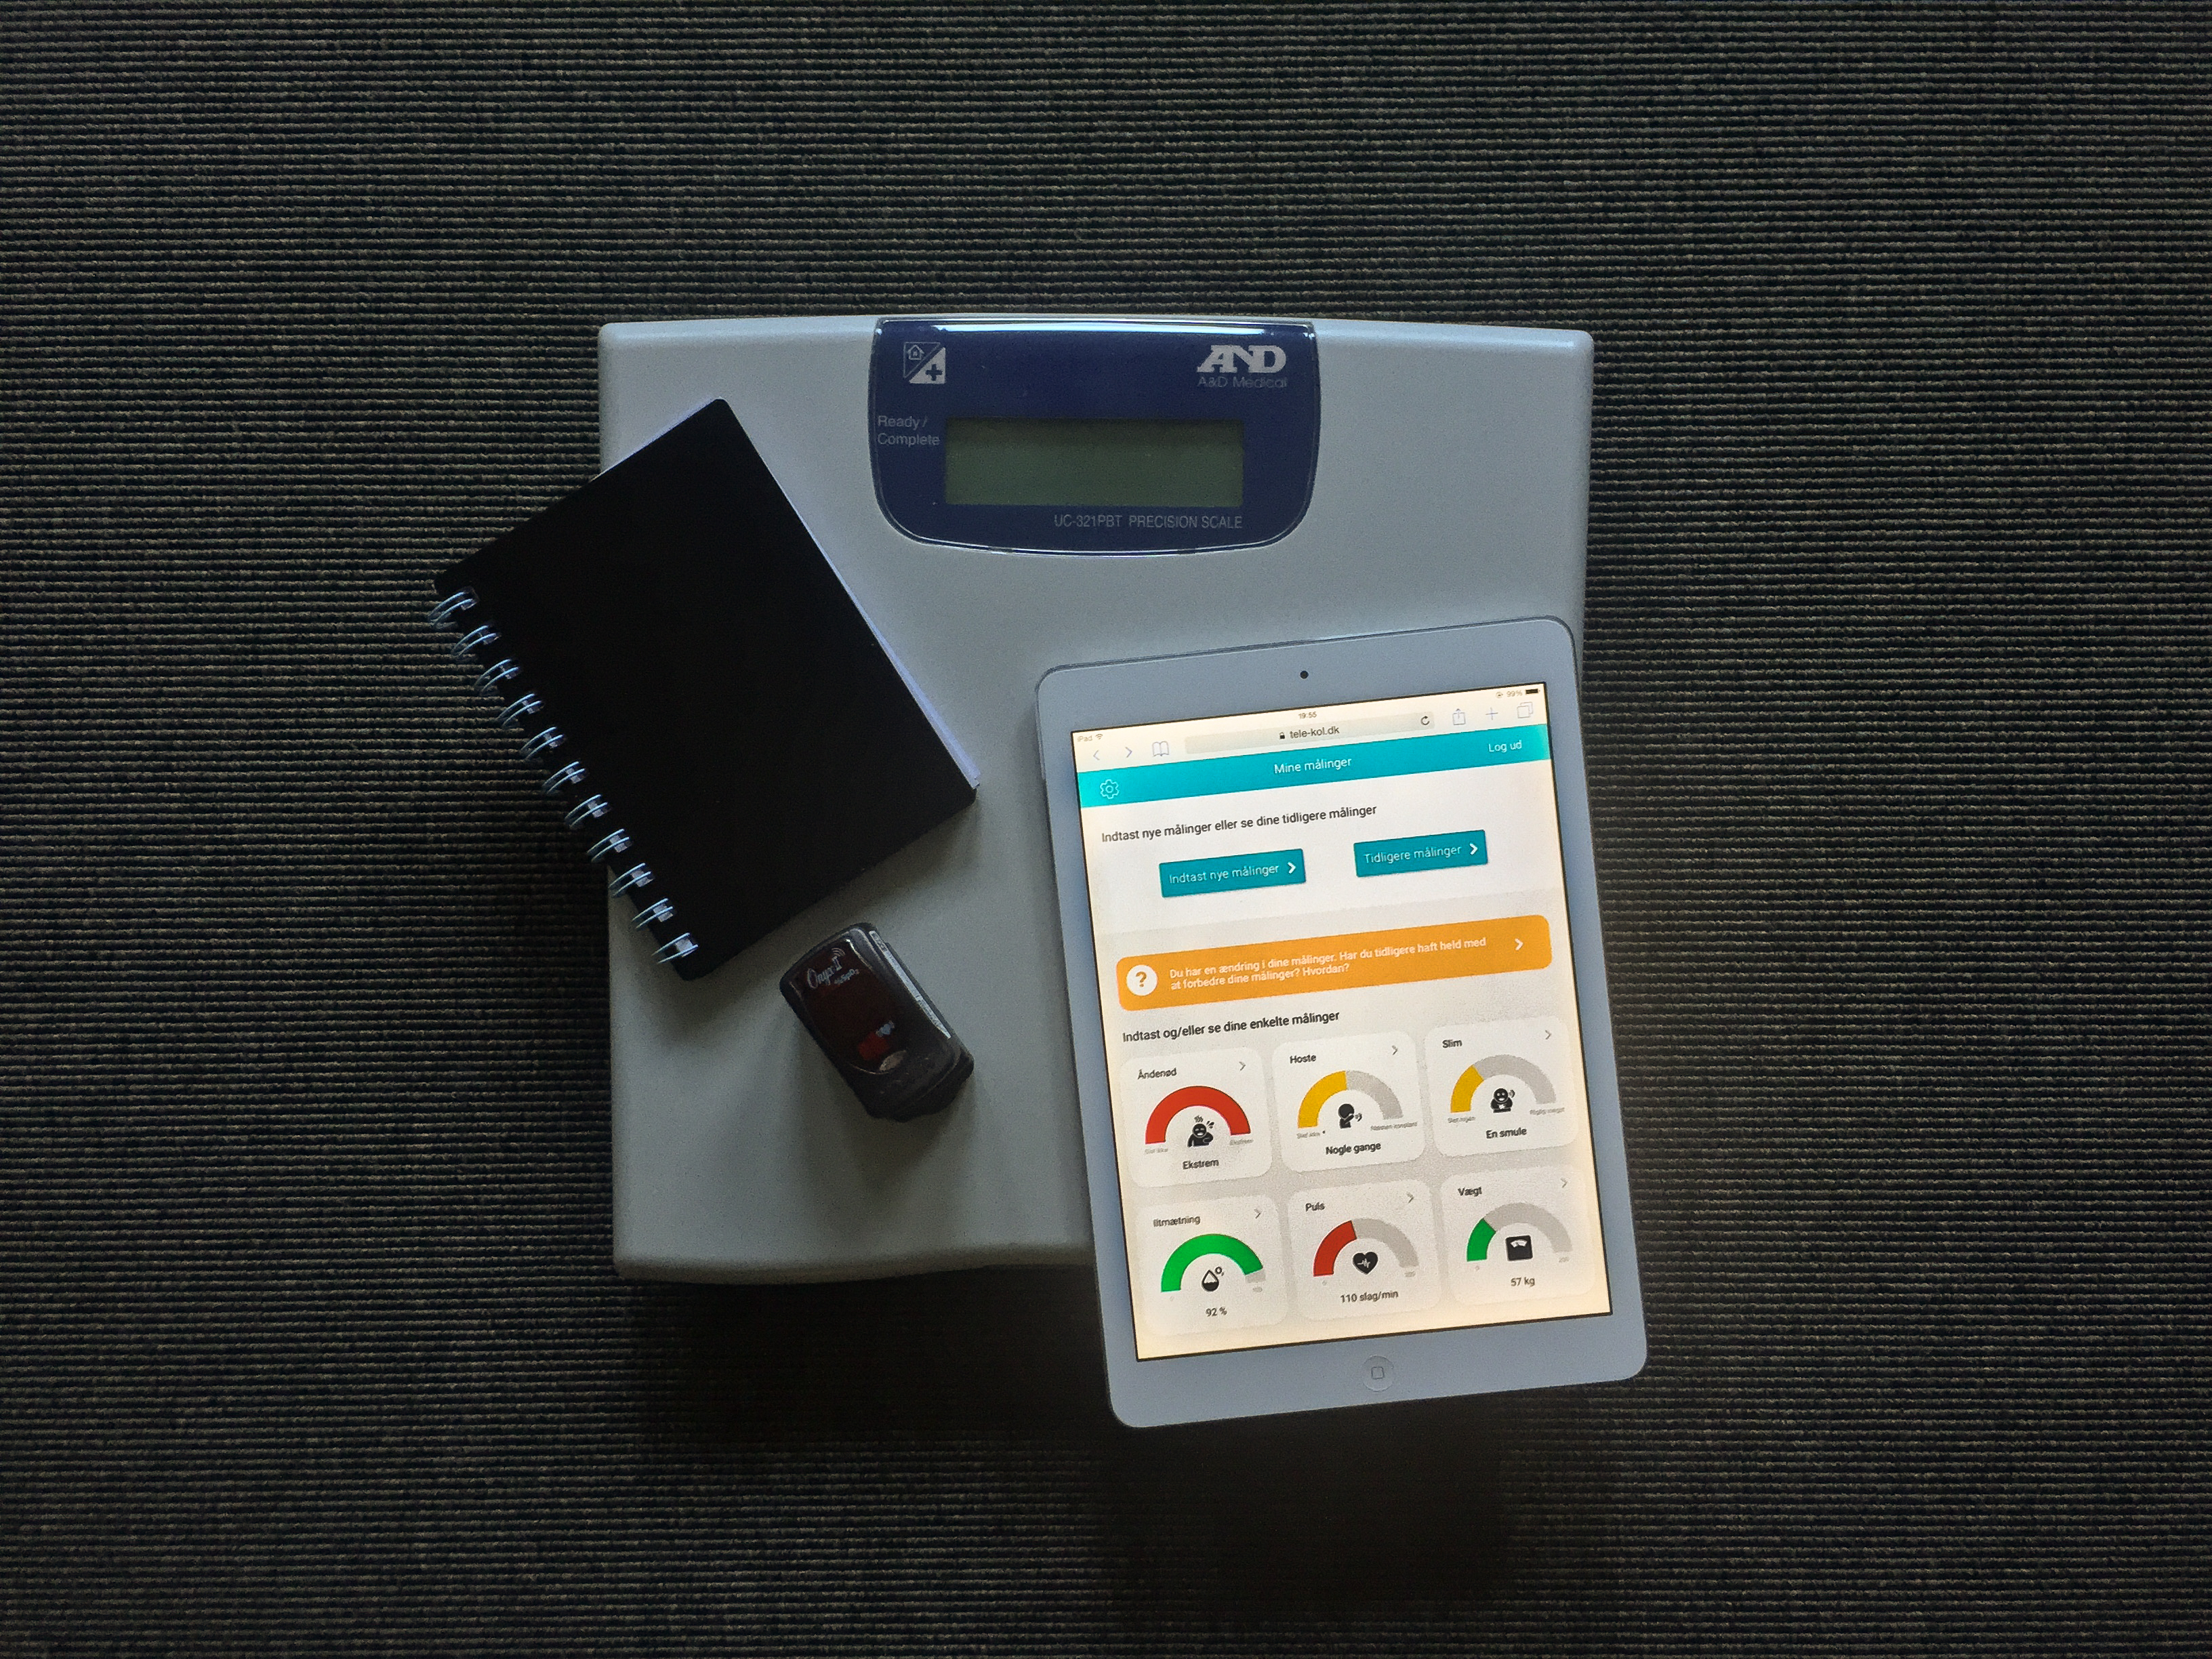
\includegraphics[width=\textwidth]{img/kit}
   %\caption{Flower two.}
 \end{minipage}
  \caption{Patient using TeleKOL (left) and TeleKOL kit (right)}~\label{fig:kit}
\end{figure}


\textit{Debriefs}: Two researchers conducted audio-recorded semi-structured interviews with all patients in their home. Each debrief lasted between 53 minutes and 1 hour and 45 minutes. Before each interview we prepared screenshots of patients' dashboard views showing events of interest (e.g. worsening or improvement in measures between two days) and summaries of log data for each patient used to cue recall in the debrief. While patients filled out demographic questionnaires, one researcher scanned the diaries for events or activities of interest and prepared interview prompts. 

The interview focused on following topics: COPD-related activities for managing disease, context of use and comparison with previous telehealth use. We showed a short video of THC to those patients, who had used it previously, to remind them (since they had not used it for a while) before we engaged in a discussion on comparing their previous telehealth experience with the system they had used. 

Inspired by the grounded theory approach \cite{IDbook}, we transcribed and coded the audio-recordings using an initial code list. We then defined emerging themes through an iterative process of reviewing the codes. We also include findings from the logging and diaries in the following. 

\subsection{Results}
From the analysis, we identified five themes: (1) Barriers for reflection and system use, (2) using measures as health status indicators, (3) feeling empowered in everyday life, (4) questioning and gaining self-knowledge and (5) becoming motivated to self-improve. While some of the themes overlap, there are also noticeable differences related to different levels of reflection. 

\subsubsection{Barriers for Reflection and System Use}
All patients mentioned the agreement with us as the main motivation for taking the system into use, except P3 who mentioned doing it, because she wanted to know her current status (\textit{self-knowledge}) and what she could do about it (\textit{self-improvement}). 

Similar to patient types found in Study 2, passive patients only took the role as data providers when using the system and did not consider it their job to engage in reflective activity of the self-tracked data. We classified three patients (P1, P3 and P4) as active patients and two patients (P2 and P5) as passive patients. 

Passive patients were not motivated to reflect on their own health, \textit{"we can not do anything except measure"} (P2) and \textit{"if the bright minds can not make sure that I get better, then neither can I do anything about it"} (P5). According to P5, reflecting on self-tracked data involved speculating about things that she did not believe she could change, \textit{"I do not worry about things that I can not change"}, but she already engaged in a similar reflective activity in order to change things, e.g. using the pulse oximeter to e.g. adjust her supplemental oxygen level, when she did not feel well.

Frequency and average duration of system use were not indicative of whether patients were classified as active or passive (See Figure \ref{charts}). All patients had used the system approximately 4-5 times, except one active patient (P4) who had used it nine times. Two of the active patients (P1, P4) logged in once during the trial period for the purpose of interacting with visualisations supporting long-term reflection alone. 

\begin{figure*}
 \centering
 \includegraphics[width=2.1\columnwidth]{img/charts}
 \caption{Frequency of use (left) and average duration of use in min/session (right)}~\label{charts}
\end{figure*}

All patients except P1 read and acted on reflective questions (e.g. system asked P4, \textit{"You have several measures that are yellow or red. Have you explored what your measures might have been affected by? (Look into previous measures)"}, wherafter P2 followed the instructions and explored multiple measures and context data). 

Patients used the system on average between 4 minutes and 51 seconds and 12 minutes and 30 seconds per session (M: 9.28), where session refers to logging in, interacting with the system and logging out. The longest session lasted 32 minutes (P4), consisting of entering measures, answering reflective question and interacting with visualisations. The shortest session lasted 3 minutes, consisting of only entering measures (P2 and P4). Both passive patients and one active patient (P3) used approximately 3/4 of the session time on the collection page. 

\subsubsection{Using Measures as Health Status Indicators}
Patients attached importance to their subjective feeling (i.e. how they are feeling) and their engagement in reflective activities on symptom changes depended on whether they felt good or bad. When patients felt good, they did not necessarily see a reason to engage in the reflective activity about symptom change. Revisiting past using the provided time series graph was not of interest to the majority of the patients, which was also reflected in the low usage among patients (except P4). 

Reflecting on the past was negatively charged by P1, \textit{"that's not something I walk around and think about .. Life gets too strenuous if you walk around and think about that [bad days in past]"} (P1). Attaching importance to embrace good days were important to patients, e.g. \textit{"[if] I actually feel good, then I do not worry about how I felt yesterday"} (P3). On the other hand not feeling well in the moment triggered reflection, \textit{"if I do not feel like everything is fine, I might start thinking why (...) it depends on how I am feeling"} (P4). 

Patients already used their pulse oximeter to check their current status, clarify whether oxygen saturation was the cause of not feeling well and then initiated action to improve their condition (e.g. breathing exercises if oxygen saturation measure was too low). The dashboard provided a similar indication of health status using multiple measures, \textit{"it [dashboard] is a measure of one's symptoms (...) altogether it of course becomes how you are feeling"} (P1). 

The self-tracking activity informed and increased the awareness of how patients were feeling, \textit{"I start noticing three times a week, how am I feeling right now?"} (P4). P3 found it helpful to have it visualised on the dashboard what caused her not feeling well, \textit{"you can not even go to the doctor and learn about your status and why (...) that you can do here [dashboard]"} (P3). 

\subsubsection{Questioning and Gaining Self-Knowledge}
In using the system, some patients had gained insights and self-knowledge that they had not previously been aware of. Patients asked themselves questions, increasing their awareness on causes of symptom changes. 

Reflective questions in combination with annotating measure with context variables in the system triggered reflection in P3, who had identified that weather had an impact on her breathing difficulties, \textit{"(..) with dyspnea, I had not thought there could be other [reasons] .. I just had breathlessness, done. (..) suddenly I realized how much I was affected by the heat (...) it happened when I sat with the system and those questions asking 'why?'"}. Annotating with context variables supported evaluating different causal explanation \textit{"I have started thinking about it (...) I think, 'no it's not that [stress]', 'Talk? No I haven't talked today' .. and then I think 'it's the weather'"} (P3).
 
P4 had started reflecting more on the day before and compared it with the presence to assess whether he could improve anything from yesterday, \textit{"I become very conscious about, how did I feel yesterday? Do I also feel like that today?"} (P4).

\subsubsection{Feeling Empowered in Everyday Life}
Using the system had a transformative effect on P3, who had obtained a new perspective on her disease after using the system and an understanding of, what the measures meant. She felt that having COPD in many years had made her passive and lost hope on being able to do something. 

\textit{"My memory has been stuck, so I thought that is just how it is.. You give up a little and get tired of it [COPD] (...) without doing anything about it, because nobody says anything.. but this [the system] does. It makes you aware about the situation (...) My doctor always told me that it is all because of my condition. The system makes me think that he is not right. I might have to make demands, then I might get better."} (P3) 

Some patients (2/5) felt more empowered in planning and overcoming everyday tasks. P3 mentioned not wanting to embarrass herself publicly and felt that she could plan to avoid such situations because of the gained knowledge about how she was affected by the heat, \textit{"now I can make up my mind beforehand [whether to go outside in the heat], because I know how it will end, now when I have been told.."} (P3). Similarly, P4 found that it provided him with a feeling of safety knowing that he was within the recommended levels in terms of his measures, which he could see on the dashboard, \textit{"I'm on the right track then. I do not have to worry about going to folk school or something else"} (P3). 

\textit{Social Responsibility:} Active patients who did not live alone (P3, P4) felt socially responsible towards their relatives. \textit{"I can become unsure about how I am feeling.. (...) I do not want to expose my husband and daughter unnecessary [frightening events] it is about balancing..I learn more about that now, so that I do not expose them [relatives]"} (P3). 

The self-tracking activity made P5 feel egocentric, but he considered it important in order to be able to do what was best for himself and his relatives, \textit{"I have to be self-centred (...) I have to do things right for myself and in time, so that I also treat others right"} (P4). 

\subsubsection{Becoming Motivated to Self-Improve}
Active patients (2/3) started setting goals themselves to improve measures. This involved seeking new knowledge, \textit{"I've tried to acquaint myself with BMI because I wanted to have a goal to follow.. [because] I wondered about the arrows [in the system]"} (P4). 

P3 had not previously been aware of the severity of her weight problems had become aware of the need of improving her condition, \textit{"I have not thought about it before, but when you suddenly get it in writing (...) being confronted with it, I have to do something about it (...) it's for my own good"} (P3). She had started making changes to her eating habits in order to lose weight (eating less, thinking about what she eats, etc.) and mentioned being more aware of engaging in proactive behaviour, \textit{"[less] coughing, that's about getting better at using the PEP device.. Not just saying, ‘oh, you are running into a pneumonia, now you have to use it', it's about using it [PEP device] several times a day"}. 

Some patients used the color indicators and arrows in combination as indicators of status and used them as goals,  \textit{"I want all of them to be green and that things are making progress"} (P3) and \textit{(...) when the arrows are pointing down I assume it is not so good, that's the wrong way"} (P4). Seeing the progress in the system and that it paid off to change her behaviours, motivated P3 to ease off medication intake, which she had tried several times in the past without success. \textit{"They had difficulties easing me off because I have had high doses for so many years (..) but this time I thought (...) now you have to stop (...) I did .. I needed some days and then it was over"} (P3). 

\textit{Actionable Advice}: Both P1 and P3 requested actionable advice on what they could do to improve their conditions. P3 needed advice on how to progress towards her goal of losing weight taking into account her other health-related conditions \textit{"to get help when you also have diabetes, that would be nice"}. P1 mentioned needing actionable advice on improving measures, \textit{"when you sit alone, have breathing difficulties, you cough and you have phlegm, you think, what can I do? It is the alpha and omega"}. 

\section{Discussion} 
We investigated how concrete design decisions regarding entry and interaction with data affected reflection in telehealth among COPD patients. Our findings indicate that active patients benefited by becoming more informed and aware about their health status using the features in the system, leading to increased empowerment in their everyday life and motivation to self-improve by setting goals. In contrast, passive patients were not interested in reflecting on their self-tracked data, but the lacking motivation to reflect on data was not a barrier for their engagement with the system (e.g. only little difference in frequency and average duration of use between active and passive patients). 

Previous literature shows conflicting results in terms of effectiveness of telehealth interventions for COPD patients on utilization of healthcare services and health-related quality of life  \cite{pedone}. We found that patients were highly motivated to log and submit data, because it provided them with sense of security to be monitored by a healthcare provider. However, we also observed an implication in current telehealth design, where some patients lacked knowledge or awareness on submitting reliable and valid measures, potentially hindering healthcare professionals in the early detection and initiation of treatment (the purpose of telehealth). 

Our findings suggest that some patients did not want to be confronted with a past that cannot be changed, whereas visualising discrepancies that can be changed, encouraged some active patients to set goals in order to self-improve. Whether patients in fact become more self-managing requires a long-term study on behaviour change. While we provided patients with visualizations of past (history data) with the purpose of supporting reflection on change over time \cite{Rivera, Cuttone} and patients mentioned benefits in seeing improvements in their measures, we found low usage of such visualizations in the real context, unless patients were curiosity-driven. Previous studies found that self-tracked data reminded people with a chronic health condition of negative aspects of their condition \cite{Li2010, Ancker2015}, which could explain our findings in relation to passive patients. Personal Informatics literature often mention simple visualisation of history as the method for supporting reflection \cite{Li2011, MacLeod2014, Rivera}, but considering the negative effects it can have on people with a deteriorating chronic condition (already suffering from anxiety and depression), we propose that future research investigates design to support seeing the positive and its effects. 

We found that designing for discrepancies (color indicators and arrows) and questioning (reflective questions in the system) triggered awareness and encouraged exploring different causal explanations (R2, higher level of reflection \cite{Fleck}) among some active patients. Whether this also makes it possible for patients to detect onsets of exacerbations earlier is yet to be investigated. It is further unclear whether outcomes will be the same, if a healthcare provider monitors the data as in real telehealth. 

Supporting previous literature on conditions for reflection \cite{Atkins, Rogers}, our findings show that passive patients were not open-minded or motivated toward engaging in reflection on their data, making it a barrier for them to benefit from the designed features. Additionally, both passive patients in the study had limited experience in interacting and using a tablet, which might have been another barrier. Fleck \& Fitzpatrick suggest that people need a reason or encouragement in order to engage in reflective activity \cite{Fleck}. In order to motivate passive patients to take a more active role in their own health, it might be necessary to consider other interventional methods or provide further support in the system to intrinsically motivate passive patients. 

Some patients were highly motivated to engage in reflection and even started setting goals to self-improve, using features in the system as goals. However, similar to Epstein et al., our findings suggest that lacking knowledge or support (e.g on how to improve measures) can be a barrier for self-improvement (action) \cite{Epstein2015}. While only three of the five participants were active and engaged in the reflective activity, the study might have been subject to self-selection bias. Particularly, the patient who gained most out of the self-tracking activity, had no previous experience with telehealth and thus no experience with the benefits of self-tracking (e.g. gaining self-knowledge). Patients might have been more reflective, because we primed them to reflect by telling them the purpose of the study and asked questions during the debriefs that prompted reflection. As mentioned by Isaac et al., reflection can be triggered when trying to externalize thoughts or feelings, e.g. in diaries. In our study, the use of diaries as a data collection method might also have fostered additional reflection \cite{Isaac}. 
 
\section{Conclusion}
Our study explores self-tracking needs in telehealth and how concrete design choices affects reflection among COPD patients. We investigated user needs and concerns critical for the effectiveness of telehealth interventions using a synthesis of literature on Personal Informatics and analysis of interviews with COPD patients using a state of the art telehealth solution. While patients generally felt taken care of, our findings show that some patients were not providing reliable and valid data, either due to lack of knowledge or awareness. Neither did the system support reflection on the self-tracked data or any follow-up action. 

Interviews, workbooks and feedback sessions informed the redesign of the telehealth system. We designed and developed a prototype to support self-reflection among the patients and evaluated it in a two week field trial. Our findings show that using simple color indicators and arrows for visualising discrepancies and asking reflective questions in the system can be a first step towards increasing active patients' self-awareness on their health status. Future researchers should investigate, how to support and motivate patients (both active and passive) e.g. through actionable advice to meet their self-tracking needs. 
